\documentclass[11pt]{beamer}
\usepackage{tikz}
\setbeamertemplate{background canvas}{\begin{tikzpicture}\node[opacity=.1]{
\includegraphics
		[width=\paperwidth]{Figuras/Capa/CirgMOdelo.png}};\end{tikzpicture}}
\usetheme{Warsaw}
\usepackage[utf8]{inputenc}
\usepackage[brazil]{babel}  % idioma
\usepackage{amsmath,amsfonts,amssymb,textcomp}
\usepackage{graphicx}
\usepackage{subfigure}
\usepackage{mathtools}
\usepackage[lined]{algorithm2e}


%% Colocando numeração nos Slides


\author{ Othon Luiz Teixeira de Oliveira }
\title[PPGES]{Defesa de Mestrado}
%\setbeamercovered{transparent} 
%\setbeamertemplate{navigation symbols}{} 
%\logo{} 
\institute{Escola Politécnica de Pernambuco -- Poli ---  UPE} 
\date{29 - Maio - 2017} 
%\subject{} 
\begin{document}


\begin{frame}
	\titlepage
\end{frame}


% Capa - requer o TikZ
\newcommand{\capa}{
    \begin{tikzpicture}[remember picture,overlay]
        \node at (current page.south west)
            {\begin{tikzpicture}[remember picture, overlay]
                \fill[shading=radial,top color=orange,bottom color=orange,middle color=yellow] (0,0) rectangle (\paperwidth,\paperheight);
            \end{tikzpicture}
          };
    \end{tikzpicture}
}

%+++++++++++++++++++++++++++++++++++++++++++++++
\begin{frame}{PPGES}
	\begin{figure}[h]
		%\left
		
\includegraphics[width=16mm, height=13mm]{Figuras/Capa/upelogo.eps}
		\qquad \quad \quad \quad \quad
		
\includegraphics[width=17mm, height=15mm]{Figuras/Capa/logoPoli.jpg}
		\qquad \quad \quad \quad \quad \quad \quad 	\vspace{0.5in}
		
\includegraphics[width=20mm, height=15mm]{Figuras/Capa/icblogo.png}
		\\
		
\includegraphics[width=55mm, height=35mm]{Figuras/Capa/logo_ppges3.png}
		
	\end{figure}
\end{frame}

\begin{frame}
	\frametitle{ \Large Programa de Pós-Graduação em Engenharia de Sistemas}
	\begin{center}
		\Large \textbf{DISSERTAÇÃO DE MESTRADO} 
	\end{center}
	\pause
	\begin{block}
		\Large \textbf{Modelo Preditivo para Sugestão de Roteamento de cargas considerando dados históricos, sócio-ambientais, e de redes sociais}
	\end{block}
	
	\pause
	\vspace{0.3in}
	%\begin{block}
	\textbf{Mestrando:} Othon Luiz Teixeira de Oliveira \\
	\textbf{Orientador:} Prof. Dr. Fernando Buarque de Lima Neto
	%\end{block}
	
\end{frame}

%%% Colocando o sumário em cada início de Sessão
\AtBeginSection[]{ 
	\begin{frame} 
		\frametitle{Sumário} \tableofcontents[currentsection, hideothersubsections] 
	\end{frame} 
} 
%%% Colocando o sumário em cada início de Subsessão
%\AtBeginSubsection[ ]{
%	\begin{frame}{Organização}
%		\tableofcontents[currentsection,currentsubsection]
%	\end{frame}
%}


%% Adiciona numeração a partir daqui, porém não parte do zero
\addtocounter{framenumber}{-1}
\setbeamertemplate
 {footline}{\quad\hfill\insertframenumber/\inserttotalframenumber\strut\quad} 

%+++++++++++++++++++++++++++++++++++++++++++++++
\section{ Introdução}
\subsection{Introdução}


\begin{frame}\frametitle{Resumo}	
	\begin{block}{O cenário}
		\begin{itemize}
			\item O transporte de cargas no Brasil é feito principalmente pelas rodovias federais (BRs). 
			\pause
			\item Essas rodovias estão constantemente congestionadas nos perímetros urbanos.
			\pause
			\item Comunidades bloqueiam as rodovias para reivindicar, dos entes públicos, todo tipo de necessidades
			\pause
			\item Em alguns trechos o traçado das rodovias está próximo a morros e florestas.
		\end{itemize}
	\end{block}
\end{frame}



%--------------------------------------------------------
%\section{ Objetivos}
\subsection{ Objetivos}

\begin{frame}\frametitle{Proposição de um modelo preditivo}
	\pause
	\begin{block}{ Objetivo Geral}
		Esta pesquisa teve como principal objetivo desenvolver um modelo de plataforma autoadaptável 
		\pause que contemple predição do comportamento das rodovias federais pernambucanas,
		\pause antecipando alguns eventos que nela possam ocorrer, apontando onde ocorrerão.
		
	\end{block}
\end{frame}

\begin{frame}\frametitle{ Objetivos Específicos}
	\pause
	\begin{block}{ Quatro objetivos}
		\begin{itemize}
			\item Caracterizar a problemática de cada rodovia;
			\pause
			\item Desenvolver um modelo preditivo dos fenômenos que envolvem as rodovias;
			\pause
			\item Desenvolver um ambiente de simulações interativas da estrutura viária em sua dinâmica
			\pause			
			\item Propor soluções para melhorar a experiência dos usuários que utilizam as rodovias pernambucanas
		\end{itemize}
		
	\end{block}
\end{frame}

\section{Background}
\subsection{Dados a minerar}

\begin{frame}\frametitle{Dados originais da PRF}
	%	\begin{block}{PRF & Twitter}
	\begin{itemize}
		\item Base de dados da Polícia Rodoviária Federal: acidente e interdições, entre 2007 a 2015.
		\pause
		\item Rede Social Twitter com 3200 tweets (limite permitido), de 2017 a 2014
	\end{itemize}	
	%	\end{block}
\end{frame}

%++++++++++++++++++++++++++++++++++++++++++++++++++++++++++++++++++++++++++++++++++++++++++++++

\begin{frame}\frametitle{ Planilha com os dados originais}
	\transboxin[duration=1, direction=25]	
	\begin{block}{ Planilha PRF}
		\begin{figure}[!ht]
			\centering %\centering % para centralizarmos a figura
			\caption{Planilha para Preprocessamento}
			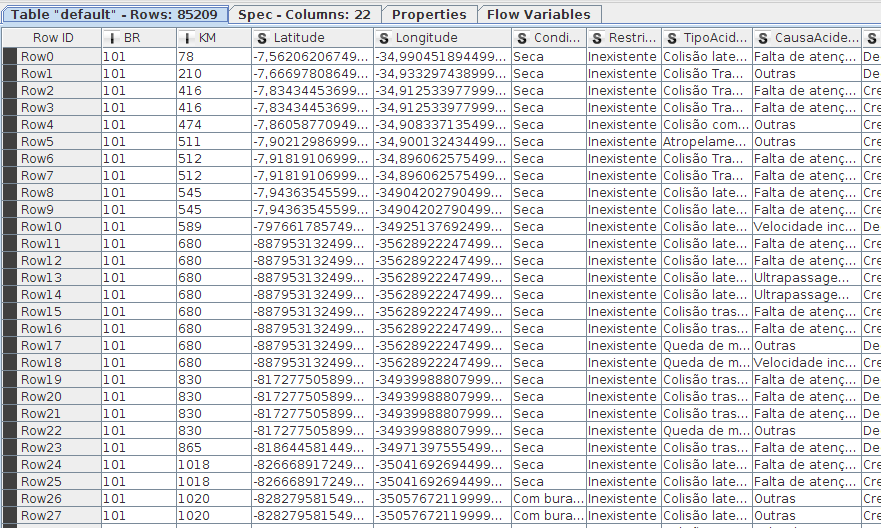
\includegraphics[width=110mm, height=40mm]{Figuras/BigData/PlanilhaPRF.png}
		\end{figure}
	\end{block}
\end{frame}


\begin{frame}
	\frametitle{ Entendendo a base de dados da PRF}
	\begin{exampleblock}{ Atributos e Instâncias -- iniciais}
		\begin{itemize}
			\item Dados de 2007 à 2015 -- BRs de Pernambuco
			\pause
			\item 85.209 Instâncias -- 27 Atributos
			\pause
			\item Dentre eles: Km, Latitude, Longitude, Condições da Pista, Causa do Acidente, Município, Data, Hora, Tipo de Veículo, Quantidade de Mortos, etc.
			\pause
			\item 40\% missing data -- 70\% do tempo total para tratar
		\end{itemize}
	\end{exampleblock}
\end{frame}

\begin{frame}\frametitle{ O Twitter}
	\begin{block}{ Acesso aos dados do Twitter}
		\begin{figure}[!ht]
			\centering %\centering % para centralizarmos a figura
			\caption{Registro de App para para acessar e baixar dados}
			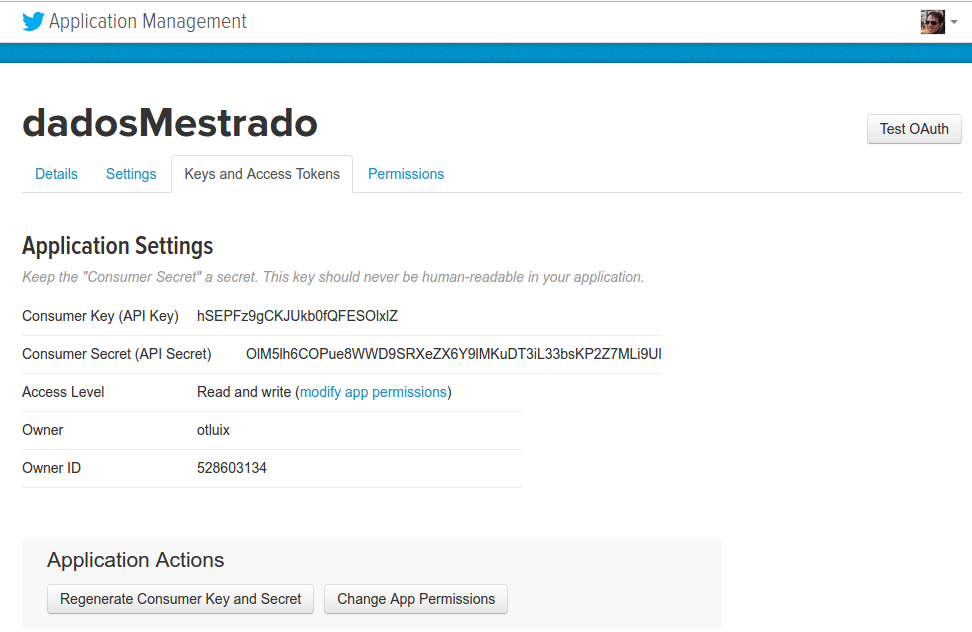
\includegraphics[width=80mm, height=35mm]{Figuras/BigData/appTweeter.png}
		\end{figure}
	\end{block}
\end{frame}

\begin{frame}\frametitle{ Dados originais}
	\transblindsvertical[duration=2, direction=25]
	\begin{block}{ Dados -- Planilha Twitter}
		\begin{figure}[!ht]
			\centering %\centering % para centralizarmos a figura
			\caption{Planilha para Preprocessamento}
			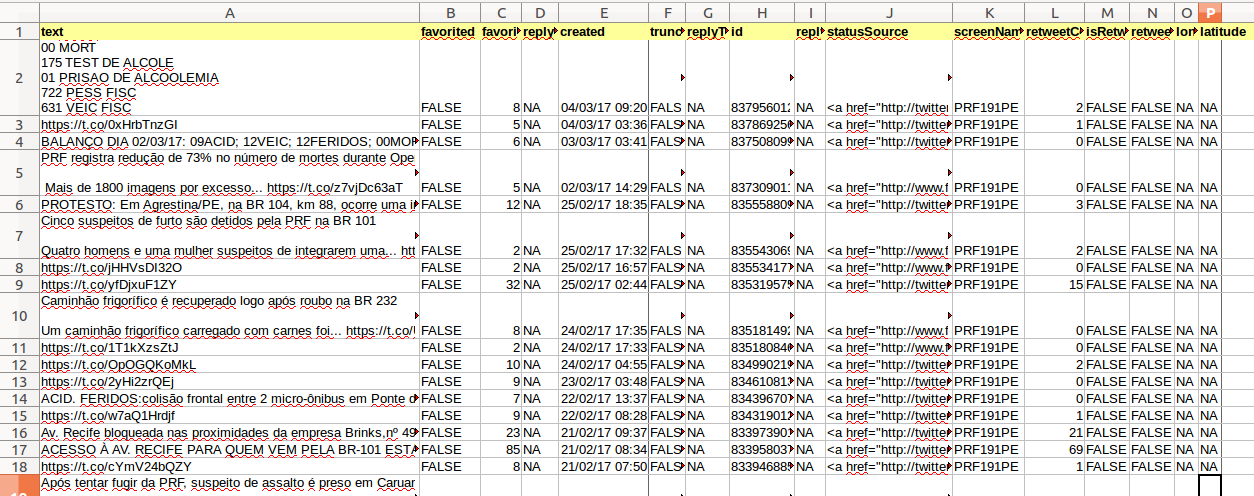
\includegraphics[width=110mm, height=40mm]{Figuras/BigData/tweetPRF.png}
		\end{figure}
	\end{block}
\end{frame}

\begin{frame}\frametitle{ Entendendo a base de dados do Twitter}
	\begin{exampleblock}{Atributos e Instâncias -- iniciais}
		\begin{itemize}
			\item Dados de 2017 -- 2014 --- canal @PRF191PE
			\pause
			\item 2864 Instâncias -- 16 Atributos
			\pause
			\item Dentre eles: 'text, 'favorited', 'favoriteConunt', 'created', 'ID', 'statusSource', 'screenName', 'retweetCount',
			\pause
			\item 'isRetweet', 'retweeted', dentre outros.		
		\end{itemize}
	\end{exampleblock}
\end{frame}

%++++++++++++++++++++++++++++++++++++++++++++++++++++++++++++++++++++++++++++++++++++++++++++++

%\section{ }
\subsection{ Metodologias de Mineração Dados --- CRISP -- DM}

\begin{frame}\frametitle{ Domínio das técnicas de Mineração de Dados}
	\transdissolve[duration=2, direction=25]
	\begin{figure}[!ht]
		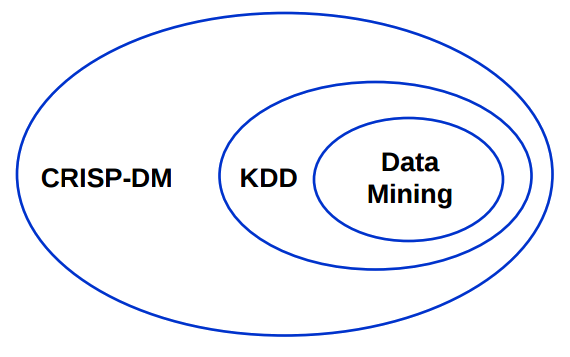
\includegraphics[width=90mm, height=60mm]{Figuras/BigData/RelacaoCrispKddDm.png}
	\end{figure}
\end{frame}


\begin{frame}\frametitle{ Cross Industry Standard Process for Data Maning -- CRISP - DM}
	\transboxout[duration=2, direction=25]
	\begin{figure}[!ht]
		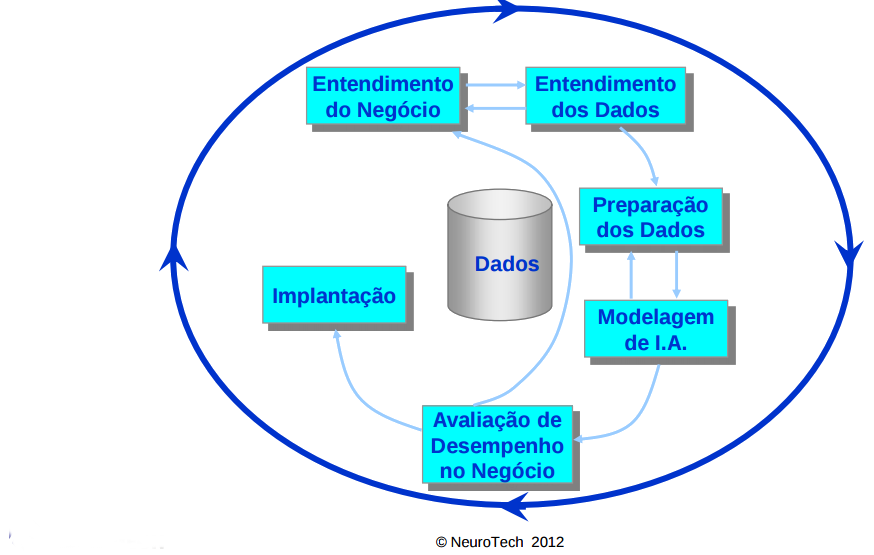
\includegraphics[width=90mm, height=60mm]{Figuras/BigData/CrispDM.png}
	\end{figure}
\end{frame}


\begin{frame}\frametitle{ Etapas CRISP-DM resumo}
	\transdissolve[duration=1, direction=25]
	\begin{figure}[!ht]
		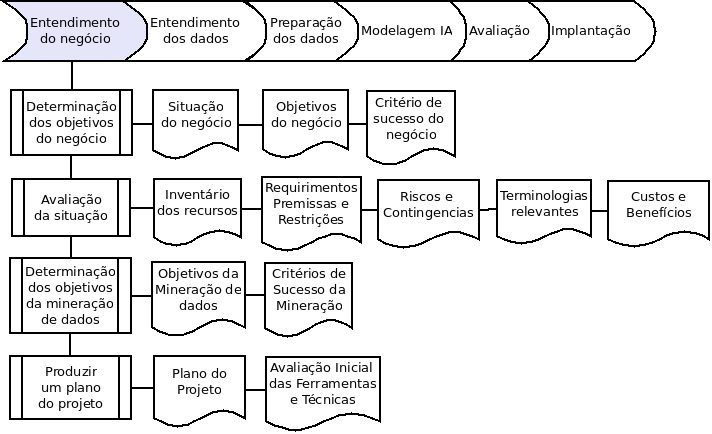
\includegraphics[width=80mm, height=58mm]{Figuras/Crisp/Entendimento.png}
	\end{figure}
\end{frame}

\begin{frame}\frametitle{ Etapas CRISP-DM resumo}
	\transdissolve[duration=1, direction=25]
	\begin{figure}[!ht]
		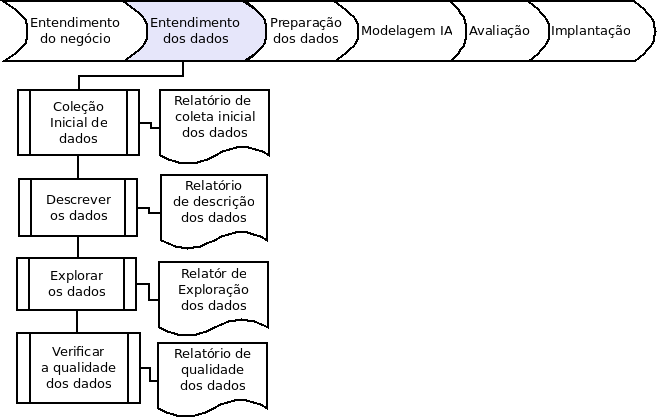
\includegraphics[width=80mm, height=58mm]{Figuras/Crisp/EntendDados.png}
	\end{figure}
\end{frame}

\begin{frame}\frametitle{ Etapas CRISP-DM resumo}
	\transdissolve[duration=1, direction=25]
	\begin{figure}[!ht]
		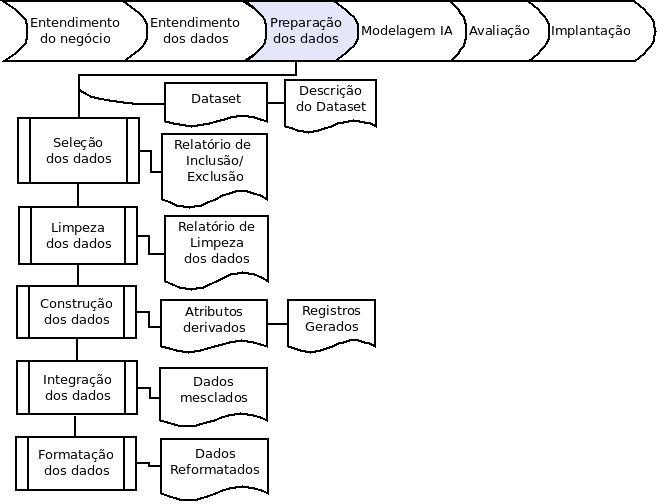
\includegraphics[width=80mm, height=58mm]{Figuras/Crisp/PreparaDados.png}
	\end{figure}
\end{frame}

\begin{frame}\frametitle{ Etapas CRISP-DM resumo}
	\transdissolve[duration=1, direction=25]
	\begin{figure}[!ht]
		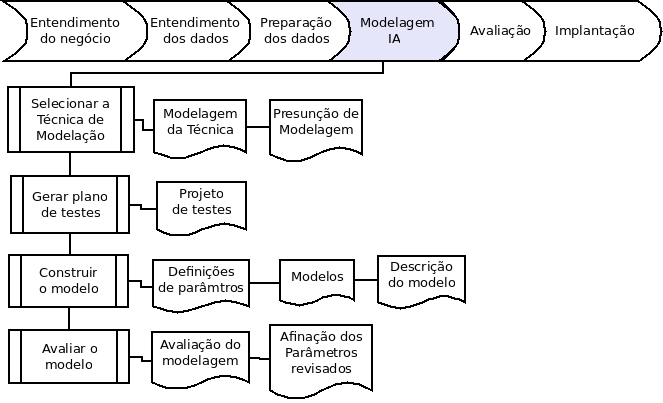
\includegraphics[width=80mm, height=58mm]{Figuras/Crisp/Model_IA.png}
	\end{figure}
\end{frame}

\begin{frame}\frametitle{ Etapas CRISP-DM resumo}
	\transdissolve[duration=1, direction=25]
	\begin{figure}[!ht]
		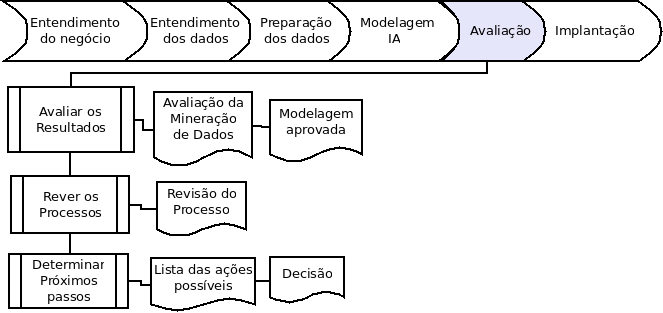
\includegraphics[width=80mm, height=58mm]{Figuras/Crisp/Avaliacao.png}
	\end{figure}
\end{frame}

\begin{frame}\frametitle{ Etapas CRISP-DM resumo}
	\transdissolve[duration=1, direction=25]
	\begin{figure}[!ht]
		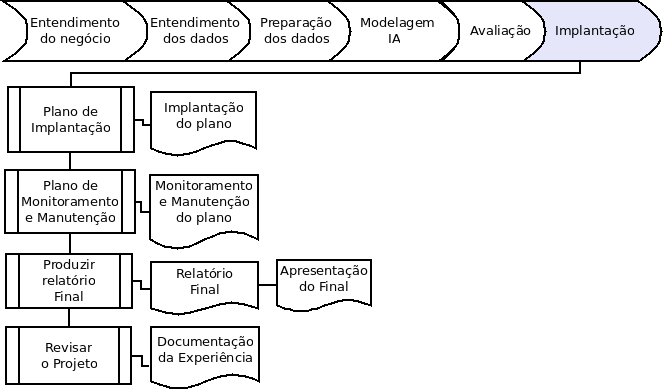
\includegraphics[width=80mm, height=58mm]{Figuras/Crisp/Implantacao.png}
	\end{figure}
\end{frame}

%\section{KDD e Mineração de Dados}
\subsection{ Minerando os dados do problema}

\begin{frame}\frametitle{ A descoberta de conhecimento (KDD) nas bases da PRF}
	\begin{figure}[!ht]
		%	\centering %\centering % para centralizarmos a figura
		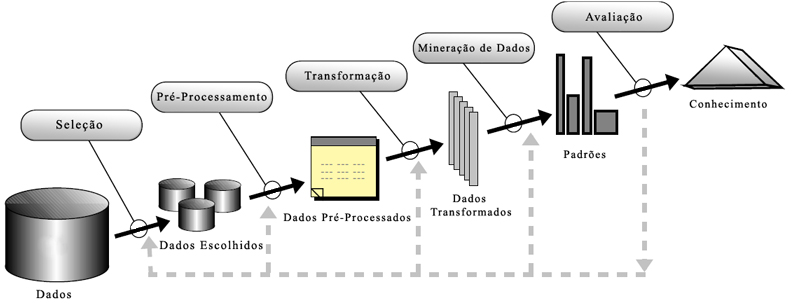
\includegraphics[width=100mm, height=30mm]{Figuras/BigData/Fayyad.png}
		\pause
		\begin{alertblock}{ Diferencça CRISP--DM --- KDD}			
			O CRISP-DM difere do KDD principalmente pelas fases do entendimento do  negócio (anterior ao KDD) e da implantação (posterior ao KDD)
		\end{alertblock}
	\end{figure}
\end{frame}


%++++++++++++++++++++++++++++++++++++++++++++++++++++++++++++++++++++++++++++++++++++++++++++++

%\section{ Tecnologias empregues na Mineração Dados}
\subsection{ Árvore de Decisão}

\begin{frame}\frametitle{ A escolha}
	\begin{exampleblock}{Pontos fortes}
		\begin{itemize}
			\item Custo benefício -- Uma árvore é gerada de maneira simples com resultados abrangente e facilidade de interpretação.
			\pause
			\item Permite fazer predição e classificação intantâneas
		\end{itemize}
	\end{exampleblock}
	\pause
	\begin{alertblock}{Pontos fracos}
		\begin{itemize}
			\item Nó raiz não é facilmente identificável
			\pause
			\item Vários testes até se conseguir resultados satisfatórios		
		\end{itemize}
	\end{alertblock}
\end{frame}


\begin{frame}\frametitle{ Cálculo da Entropia e Entropia Condicional}
	\transdissolve[duration=1, direction=25]
	\centering{Equação da entropia}
	\begin{equation}
	H_{x}=-\sum_{\forall x \in X}P(x)log_{2}P(x)
	\end{equation}
	\centering{Equação da entropia condicional}
	\begin{equation}
	H_{Y|X}= \sum_{x}P(x)H(Y|X=x) =-\sum_{\forall x \in X}P(x) \sum_{\forall y \in Y}P(y|x)log_{2}P(y|x)
	\end{equation}
\end{frame}


\subsection{ Naïve Bayes}

\begin{frame}\frametitle{ Teorema de Bayes e Aprendizagem bayesiana}
	\transdissolve[duration=1, direction=25]
	\centering{Teorema de Bayes: forma tradicional}
	\begin{equation}
	p(C_{k}|x) = \frac{p(_{k})p(x|C_{k})}{p(x)}
	\end{equation}
	
	\centering{Teorema de Bayes: forma simplificada}
	\begin{equation}
	p(posteriori) = \frac{p(priori) * {\text{verossimilhança}}}{\text{evidência}}
	\end{equation}
\end{frame}

\subsection{ Redes Neurais}

\begin{frame}\frametitle{ Classificação com Redes Neurais}
	\transdissolve[duration=1, direction=25]
	Rede Nerual com três camadas identificadas
	\begin{itemize}
		\item Camada de entrada: apresenta-se os padrões à rede
		\item Camada intermediária (ocultas): realiza a maior parte do processamento por conexões ponderadas
		\item Camada de saída: conclusão e apresentação do resultado.
	\end{itemize}
	\begin{figure}[!ht]
		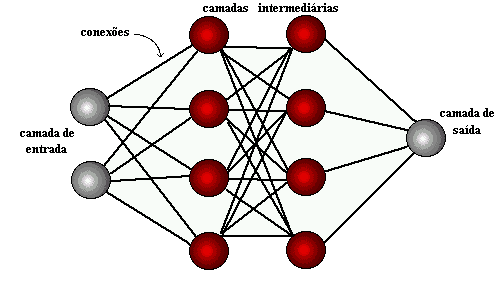
\includegraphics[width=80mm, height=40mm]{Figuras/BigData/camdasIntermediarias.png}
	\end{figure}
\end{frame}

%++++++++++++++++++++++++++++++++++++++++++++++++++++++++++++++++++++++++++++++++++++++++++++++

%\section{ Mineração em Textos}
\subsection{ Tecnologias empregues na Mineração em Textos}

\begin{frame}\frametitle{ TF -- IDF}
	\transdissolve[duration=1, direction=25]
	 \centering{Text Frequence X Inverse Document Frequence: $TF * IDF$}
	\begin{equation}
		idf(term) = \ln(\frac{n_{documents}}{n_{documents\  containing \ term}})
	\end{equation}
	\pause
	\begin{figure}[!ht]
	 		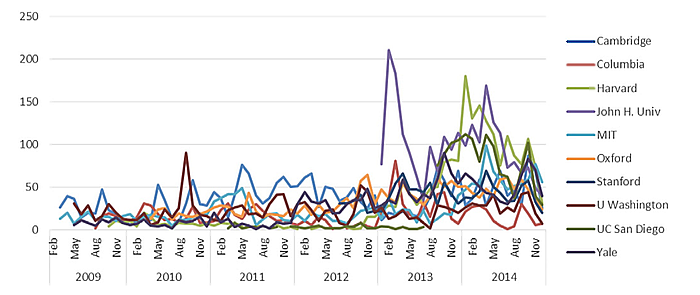
\includegraphics[width=70mm, height=40mm]{Figuras/BigData/ferqPalavrasG.png}
	\end{figure}
\end{frame}

\subsection{ Análise de Desempenho aplicados à mineração}
\begin{frame}\frametitle{AUC -- Matriz Confusão}

	A área sob a curva AUC (Area under ROC -- Reciver Operating Characeteristic) é uma métrica que determina a qualidade do classificador.
	Ela é calculada cruzando-se verdadeiros positivos com os falso positivos. 
	Esta área varia entre zero e um, quanto mais próximo de 1(um) o classificador conseguiu acertar mais vezes do que errar.
	A seguir a Matriz de Confusão que agrupa essas atributos.
	%tabela 5
	\begin{table}[ht]
		\centering
		\caption{Matriz de Confusão}
		\vspace{1mm}
		\begin{tabular}{l|c|c}
			\hline
			\textbf{} & \textbf{Predito} & \textbf{}\\
			\hline
			\textbf{Real}  & TP   FN & Positive -- POS\\
			\textbf{Real}  & FP   TN & Negative -- NEG\\
			\hline
			---         & PP   PN &    ---         \\
		\end{tabular}
		\\
		\tiny Fonte: Bradley -- 1997
	\end{table}
\end{frame}

\begin{frame}\frametitle{ Análise de Desempenho aplicados à mineração}
	
	A Matriz Modelo de Confusão sintetiza a Matriz modelo de Confusão.
%tabela 6
\begin{table}[ht]
	\centering
	\caption{Matriz modelo de Confusão}
	\vspace{1mm}
	\begin{tabular}{l|c|c}
		\hline
		\textbf{}           & \textbf{Y}     \textbf{$\bar{Y}$}   & \textbf{}\\
		\hline
		\textbf{X}          & P(X,Y)         P(X,$\bar{Y}$)       & Positive -- POS\\
		\textbf{$\bar{X}$}  & P($\bar{X}$,Y) P($\bar{X},\bar{Y}$) & Negative -- NEG\\
		\hline
		---              & P(Y)           P($\bar{Y}$)         &     ---        \\
	\end{tabular}
	\\
	\tiny Fonte: Bradley -- 1997
\end{table}

 Para construir a curva ROC utiliza-se as probabilidades condicionais cruzando-se a taxa de verdadeiros positivos ($ tpr = P(Y|X)$) probabilidade de falsos alarmes ou taxa de falsos positivos será ($ fpr = P(Y,\bar{X})$),
 
 
\end{frame}
%++++++++++++++++++++++++++++++++++++++++++++++++++++++++++++++++++++++++++++++++++++++++++++++

\section{Contribuição}
\subsection{Nossa contribuição}
\begin{frame}
	\frametitle{Contribuição}
	 Nossa contribuição:
	 \begin{itemize}
	 	\item Do ponto de vista metodológico: Aplicação do processo CRISP-DM a uma abordagem que integre predição e classificação;
	 	\pause
	 	\item Do ponto de vista prático: Integração entre mineração de dados e mineração em textos.
	 \end{itemize}.
\end{frame}

\begin{frame}
	\frametitle{Aplicação dos algorítmos de IA}
	
	\begin{itemize}
		\item Para classificação foram empregues: Árvores de Decisão e Naïve Bayes;
		\pause
		\item Para predição a priori utilizou-se Redes neurais.
		\pause
		\item Os algoritmo escolhidos contemplam características especiais tais como: robustez, tolerância a ``missing data'', aprendizagem e facilidade de interpretação.
	\end{itemize}.
\end{frame}


\begin{frame}
	\frametitle{Aplicação dos algorítmos de IA, continuação}
	\begin{itemize}
		\item Propomos a integração de APIs de mapas de posicionamento global;
		\pause
		\item Integração de APIs de redes sociais formando um arco cibernético com essas informações melhorando a experiência do utilizador.
		\pause
		\item Soluções conhecidas: Wase, Google Maps e outros não analisam dados históricos nem analisam outras redes sociais, também não integram tudo em uma única ferramenta.
	\end{itemize}.
\end{frame}

\subsection{Modelo Proposto}
\begin{frame}
	\frametitle{O Modelo proposto}
	\begin{itemize}
		\item A primeira fase da nossa metodologia contempla todas as fases do CRISP-DM, classificação, predição e descoberta de conhecimento nas bases históricas;
		\pause
		\item Para predição a priori utilizou-se Redes neurais;
		\pause
		\item Para extrapolação do modelo preditivo ocorre quando este se integra a APIs de mapas vetoriais, disparado pelo agente: utilizador.
	\end{itemize}.
\end{frame}

\begin{frame}\frametitle{ Representação gráfica do modelo preditivo e da extrapolação}
	\transboxout[duration=2, direction=25]
	\begin{figure}[ht]
		\centering
		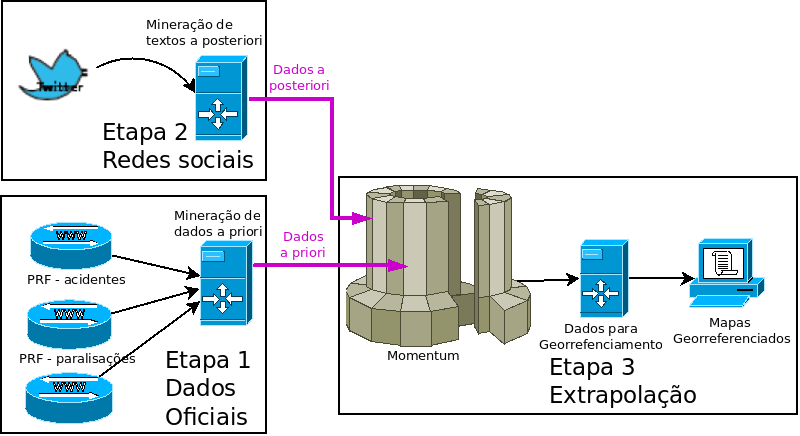
\includegraphics[width=100mm, height=50mm]{Figuras/Metodologia/metodologiaGeral3.png}
		\caption{Etapas do modelo preditivo e extrapolação}		
	\end{figure}
\end{frame}

\begin{frame}\frametitle{ Etapa 1 -- Dados oficiais}
%	\transboxout[duration=1, direction=25]
 A primeira etapa, \textit{a priori}, contempla os dados da PRF
 Esses dados foram tratados, variáveis foram transformadas em:\begin{table}[htbp!]
 	\centering
 	\caption{Variáveis transformadas} 
 	\begin{tabular}{r|l} \hline
 		KMarred & Numeração do quilômetro arredondada \\
 		BRajusta & Nome da BR literal\\
 		CondPista & Condição da pista: seca, molhada, ... \\
 		RestriVisibili & Restrição de visibilidade: inexistente,... \\
 		TipoAcid & Tipo de Acidente: atropelamento, colisão...\\
 		CausaAcid & A possível causa do acidente: Falta de... \\
 		TracadoVia & Tipo de traçado da via: reta, curva,... \\
 	\end{tabular}
 \end{table}
\end{frame}

\begin{frame}\frametitle{ Etapa 1 -- continuação..}
	\begin{table}[htbp!]
		\centering
	 	\caption{Variáveis transformadas} 
		 \begin{tabular}{r|l} \hline 
		 		Tipo veículo & Tipo de veículo envolvido no acidente \\
		 		DiaSemana & Dia em que ocorreu o acidente\\
		 		Hora & Horário do acidente/ocorrência: hh:mm \\
		 		QtdMortos & Quantidade de mortos envolvidos \\
		 		Gravidade & Quantidade de acidentes graves \\
		 		Período & Turno do dia em que se deu a ocorrência \\
		\end{tabular}
	\end{table}
\end{frame}

\begin{frame}\frametitle{ Extração do conhecimento -- KDD}
	\begin{itemize}
		\item Optamos por coletar os dados diretamente dos órgãos oficias, devido a não padronização dos dados. A PRF possui ao menos dois bancos de dados: de acidentes e de interdições.
		\pause
		\item Após a integração dessas bases e seguidas as etapas de Mineração procedeu-se a extração do conhecimento.
		\pause
		\item Para traçar um painel da diversidade das rodovias, foi feito, a priori, uma classificação com AD e comparado com NB.
		\pause
		\item Foi escolhida a variável BRajustada porque esta continha alta de correlação linear e a entropia satisfatórias, produzindo altas taxas de classificação.
		\pause
		\item Por conseguinte partimos para a proposição de uma representação do conhecimento adquirido.  
	\end{itemize}
\end{frame}

\subsection{ As Matrizes}
\begin{frame}\frametitle{ Matriz de Mortos}
	A Matriz de Mortos contém todos os óbitos registrado pela PRF, em cada trecho de cada rodovia, a cada hora do dia.
	\pause
	\transboxin[duration=1, direction=25]
	\begin{figure}[!ht]
		\centering
		\label{fig:MatrizMortos2D}
		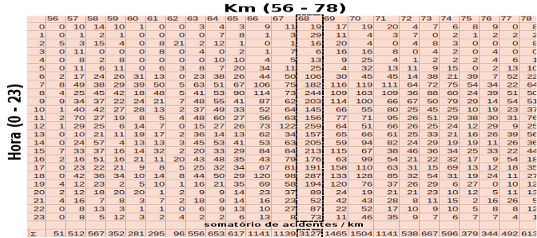
\includegraphics[width=110mm, height=50mm]{Figuras/Metodologia/MM2d101.png}\\
		\caption{Matriz de Mortos 2D - BR 101, Período: 2007 à 2015}
	\end{figure}
\end{frame}

\begin{frame}\frametitle{ Matriz de Gravidade3D}
	A Matriz de Gravidade3D contempla uma maior variabilidade das ocorrência nos pontos que a Matriz de Mortos não detectou.
	\pause
	\transboxin[duration=1, direction=25]
	\begin{figure}[!ht]
		\centering
		\label{fig:MatrizMortos2D}
		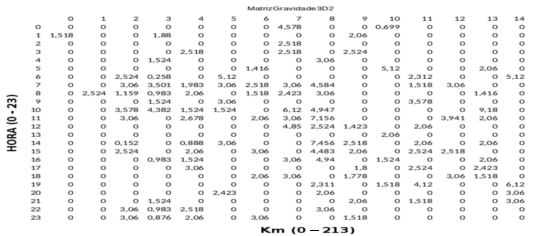
\includegraphics[width=110mm, height=50mm]{Figuras/Metodologia/MatrizGravidade3D2.png}\\
		\caption{Matriz de Gravidade3D - BR 101, Período: 2007 à 2015}
	\end{figure}
\end{frame}

\begin{frame}\frametitle{ Matriz de Gravidade3D}
	Cruzando-se $< km, Hora >$ de cada Matriz temos um ponto de ocorrência. Na Matriz de Gravidade3D esses pontos foram encontrado segundo a equação de probabilidades (BR 101):
\pause
\begin{equation}
ProbAcid_{101} = (RestVisibi + CondPista + TracadoVia) *  Erro_{101} + Gravidade
\end{equation} 
\pause
Onde:
\begin{itemize}
	\item RestVisibi - Restrição de Visibilidade;
	\item CondPista  - Condição da Pista;
	\item TraçadoVia - Traçado da Via;
	\item Erro\_\{101\} - Taxa de Erro da AD para a BR 101
	\item Gravidade - Ocorrência de óbito (variável binarizada)
\end{itemize}
\end{frame}


\subsection{O Twitter}
\begin{frame}\frametitle{ Arco cibernético com dados do Twitter}
Os dados do Twitter permitem buscar informações no momento em que o utilizador iniciar sua viagem. 
\pause
Verificamos que predições como protestos, queda/remoção de barreiras e rochas são sazonais em Pernambuco, portanto não estão contemplados no modelo de predição.
\pause
\begin{figure}[ht]
	\centering
	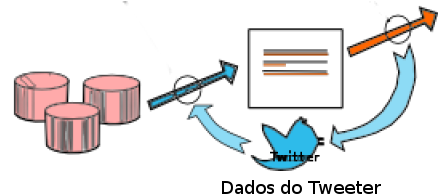
\includegraphics[width=70mm, height=30mm]{Figuras/Metodologia/ArcoCibernetico.png}\\
	\caption{Arco cibernético com dados do Twitter}
\end{figure}
\end{frame}

\subsection{Extrapolação para georreferenciamento}
\begin{frame}
	\frametitle{ Localizando os pontos críticos}
	As matrizes apresentadas (Mortos e Gravidade) representam pontos críticos nas rodovias. Esses pontos podem ser extrapolados em coordenadas geográficas para mapas de georreferenciamento.
	\pause
  \begin{figure}[ht]
	\centering
	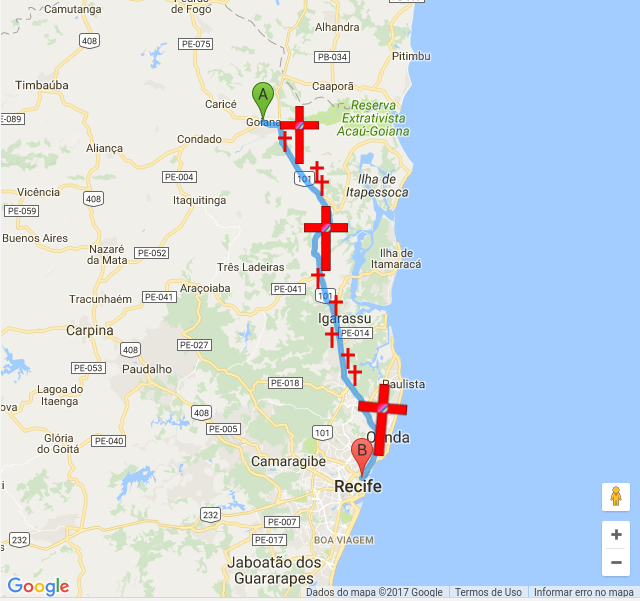
\includegraphics[width=80mm, height=40mm]{Figuras/Metodologia/georreferenciamento.png}\\
	\caption{Etapas 3 -- Georreferenciamento}
  \end{figure}
\end{frame}

%++++++++++++++++++++++++++++++++++++++++++++++++++++++++++++++++++++++++++++++++++++++++++++++
\section{Resultados}
\subsection{Execução do Modelo}
%1

\begin{frame}
	\frametitle{ Visão geral do Modelo Proposto}
	\begin{figure}[ht]
		\centering
		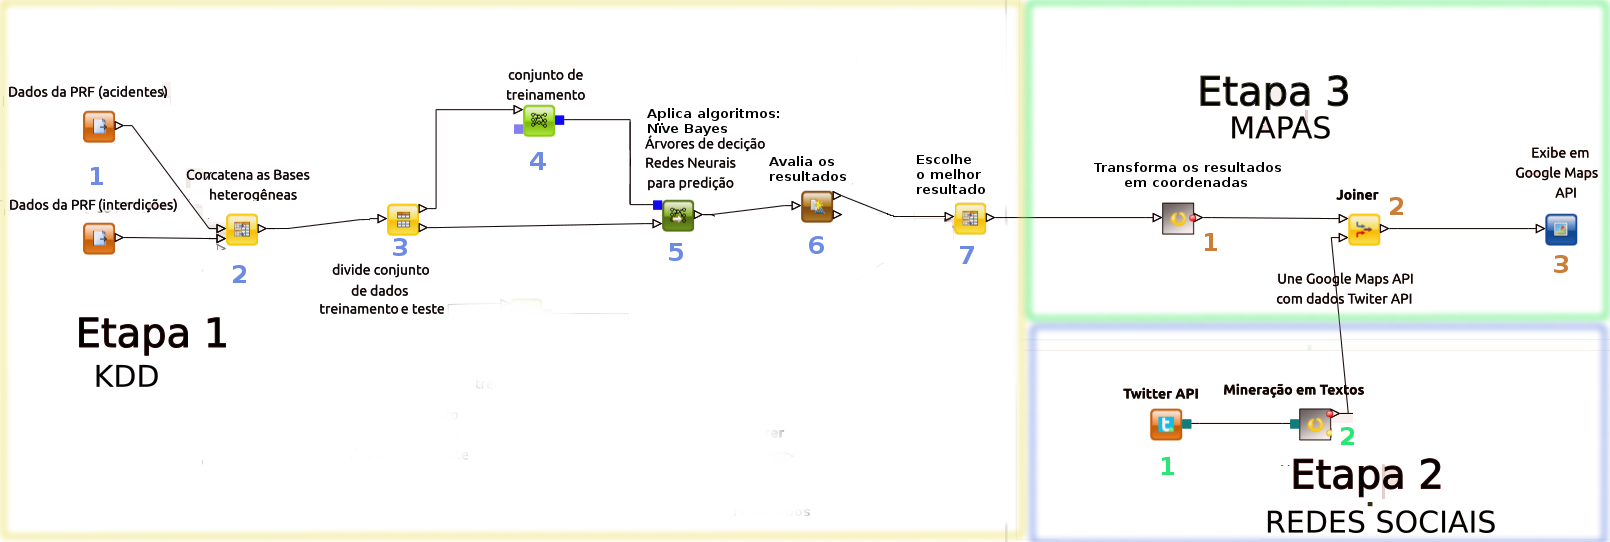
\includegraphics[width=100mm, height=50mm]{Figuras/Resultados/metodologia.png}\\
		\caption{Etapas do modelo proposto}
	\end{figure}
\end{frame}
%2

\begin{frame}
	\frametitle{A Etapa 1 -- KDD}
	O KDD contempla a fase de coleta da bases históricas, preparação e execução dos algoritmos e descoberta dos pontos críticos descrito a seguir:
	\pause
	\begin{enumerate}
		\item O modelo preditivo integra as bases de dados da PRF;
		\pause
		\item As bases são concatenados de acordo com a lógica do negócio;
		\pause
		\item Tratamento e divisão dos dados em: conj. de treinamento e testes;
		\pause
		\item Treina e Executa os algoritmos de IA escolhidos;
		\pause
		\item Caso os algoritmos não tenham produzidos os resultados esperados ocorre extração de conhecimento.
		\pause
		\item Análise das métricas: AUC e Matriz de Confusão.
		\pause
		\item Escolha dos melhores: AUC, Inst. Classif. corretamente, Inst. classif. incorretamente e Erro médio absoluto.
	\end{enumerate}
\end{frame}
%3

\begin{frame}
	\frametitle{A Etapa 2 -- Redes Sociais}
	Esta etapa é um modulo dinâmico e analisa momentaneamente os feeds postados pelos usuários das redes sociais;
	\pause
 \begin{enumerate}
 	\item São capturados ``feeds'' da rede social Twitter (para esta pesquisa). 
 	Essa técnica faz um arco cibernético mantendo o utilizador atualizado com as informações recentes.
 	\pause
 	\item Após a captação dos dados do Twitter é feita a Mineração nos textos para localizar informações que permitam antever alguma paralização futura nas rodovias. 
 \end{enumerate}
\end{frame}
%4

\begin{frame}
	\frametitle{Etapa 3 -- Integração de APIs}
  \begin{enumerate}
	\item Conversão dos melhores resultados encontrados na Etapa 1 $<Km, Hora>$ em coordenadas;
	\pause
	\item Localizações geográficas dos pontos críticos da malha viária, indicadas pelo Km, são agrupadas formando ''clusters`` de dados exibidos em mapas vetoriais. Une API do Google Mapas e API do Twitter;
	\pause
	\item Exibe informações vindas do twitter sobre ocorrências na rodovia, encontrando sua geolocalização a ser transformado em marcos ``milestone'' para representação sobre mapas de bases vetoriais.
  \end{enumerate}
\end{frame}
%5
\subsection{Análise das Rodovias -- Antes da MD}

\begin{frame}\frametitle{Dados encontrados para a BR 101}
  O dados revelaram que a grande maioria dos acidentes ocorre com pista seca, sem restrição de visibilidade e em linha reta.
  A seguir gráficos da BR 101, em vermelho são os pontos críticos, em azul com menos frequência de acidentes.
	\pause
  \begin{figure}[h]
	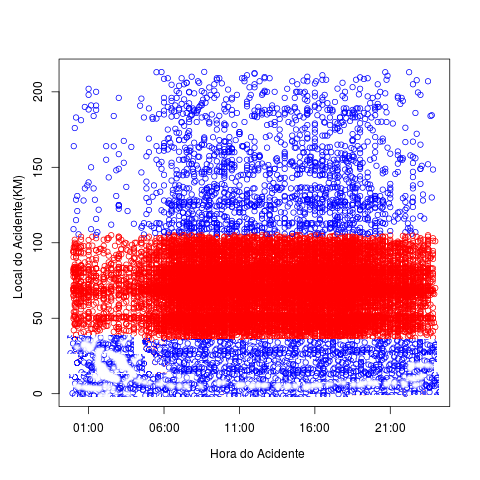
\includegraphics[width=3.5cm,height=3.5cm]{Figuras/Preprocess/br101.png}
	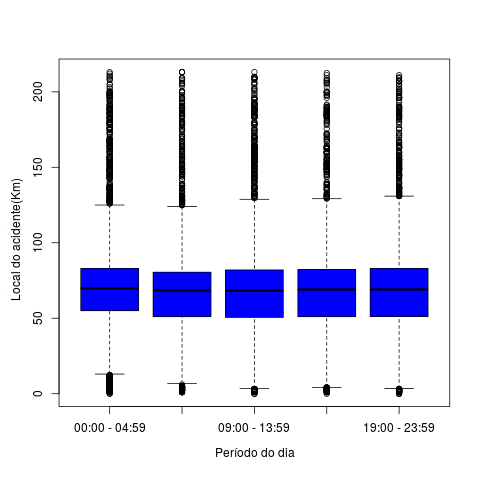
\includegraphics[width=3.5cm,height=3.5cm]{Figuras/Preprocess/br101_2.png}
	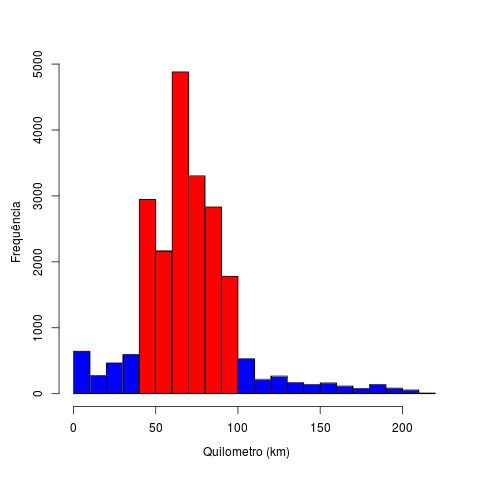
\includegraphics[width=3.5cm,height=3.5cm]{Figuras/Preprocess/br101_4.png}
	\caption{BR 101: Hora do acidente (1) Concentração em torno da hora (2) e Frequência (3)}
  \end{figure}
\end{frame}
%6

\begin{frame}\frametitle{Dados encontrados para a BR 104}
	Conhecida como rota da sulanca esta rodovia apresenta concentração de acidentes entre o km 60 e 70
	\pause
	\begin{figure}[h]
		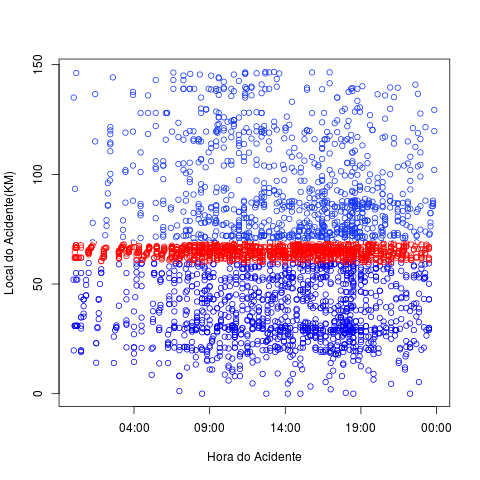
\includegraphics[width=3.5cm,height=3.5cm]{Figuras/Preprocess/br104_12.png}
		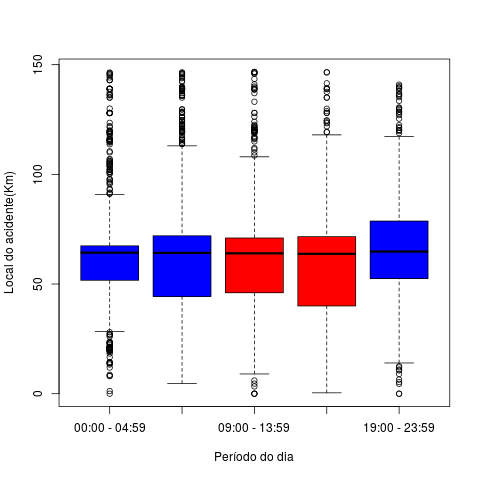
\includegraphics[width=3.5cm,height=3.5cm]{Figuras/Preprocess/br104_2.png}
		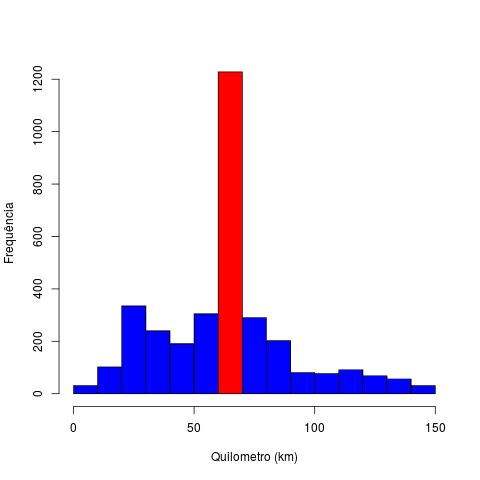
\includegraphics[width=3.5cm,height=3.5cm]{Figuras/Preprocess/br104_3.png}
		\caption{BR 104: Hora do acidente (1) Concentração em torno da hora (2) e Frequência (3)}
	\end{figure}
\end{frame}
%7
%\subsection{Extrapolação para georreferenciamento}
\begin{frame}\frametitle{Dados encontrados após a MD}
	Resultados dos Classificadores:
	As variáveis ``TipoAcidente'', ``Gravidade'' e ``BRajustada'' obtiveram a melhor relação ganho de informação.
	A métrica para avaliar os resultados dos classificadores foram:
	\pause
  \begin{itemize}
	\item TP: True Positive;
	\item FP: False Positive;
	\item Prec.: Precison = TP/(TP +FP);
	\item Recall = TP/ (TP + FN);
	\item F-Me: F-measure ou f-score = 2 * Precison * Recall / (Precision + Recall);
	\item AUC: Area Under Curve (Roc);
  \end{itemize}
\end{frame}
%8
%\subsection{Extrapolação para georreferenciamento}
\begin{frame}\frametitle{Comparando as métricas para a variável BRajustada}
	Resultado obtido pela AD:
	\begin{table}[!ht]
		\centering
		%\caption{Volume de dados no mundo}
		\vspace{1mm}
		\begin{tabular}{l|c|c}
			\hline
			\textbf{Descrição} & \textbf{Valores} & \textbf{Percentual} \\
			\hline
			Instâncias Corretamente Classificadas & 13507 & 80.5522\% \\
			Instâncias Incorretamente Classificadas & 3261 & 19.4478\% \\
			Erro médio quadratico & 0.1656 & --- \\
		\end{tabular}
\pause
	\end{table}
	Resultado obtido pelo NB:
		\begin{table}[!ht]
			\centering
		%	\caption{Instâncias classificadas e Erro médio}
			\vspace{1mm}
			\begin{tabular}{l|c|c}
				\hline
				\textbf{Descrição} & \textbf{Valores} & \textbf{Percentual} \\
				\hline
				Instâncias Corretamente Classificadas & 9232 & 73,3339\% \\
				Instâncias Incorretamente Classificadas & 3357 & 26,6661\% \\
				Erro médio quadrático & 0.1908 & --- \\
			\end{tabular}
		\end{table}
\end{frame}
%9
\begin{frame}\frametitle{Matriz de Confusão para a variável BRajustada encontrada pela AD}
	\begin{table}[!ht]
		\centering
	%	\caption{Matriz de confusão para a variável BRajustada}
		\vspace{1mm}
		\begin{tabular}{l|c|c|c|c|c|c|c|l}
			\hline
			\textbf{a} & \textbf{b} & \textbf{c} & \textbf{d} & \textbf{e} & \textbf{f} & \textbf{g} & \textbf{h} & \textbf{Classificadas}\\
			\hline
			6960 & 0 & 0 & 625 & 0 & 0 & 0 & 0 & BR101 \\
			0 & 1071 & 0 & 156 & 0 & 0 & 0 & 0  & BR104 \\
			0 & 0 & 0 & 625 & 0 & 0 & 26 & 11  & BR110 \\
			0 & 0 & 85 & 0 & 90 & 11 & 0 & 0  & BR116 \\
			970 & 9 & 0 & 3185 & 1 & 0 & 1 & 0  & BR232 \\
			0 & 0 & 27 & 11 & 377 & 7 & 0 & 0  & BR316 \\
			0 & 0 & 0 & 0 & 0 & 95 & 0 & 0  & BR407 \\
			643 & 0 & 0 & 66 & 0 & 0 & 0 & 0  & BR408 \\
		%	0 & 39 & 0 & 0 & 0 & 0 & 449 & 92  & BR423 \\
		%	0 & 0 & 0 & 625 & 0 & 0 & 172 & 154  & BR424 \\
		%	0 & 0 & 15 & 0 & 3 & 675 & 0 & 0  & BR428 \\			
		\end{tabular}
	\end{table}
\end{frame}

%10
\begin{frame}\frametitle{Matriz de Confusão para a variável BRajustada encontrada pelo NB}
%	Resultado obtido pela NB:
	\begin{table}[!ht]
		\centering
%	\caption{Matriz de confusão -- BRajustada -- Naïve Bayes}
		\vspace{1mm}
		\begin{tabular}{l|c|c|c|c|c|c|c|l}
			\hline
			\textbf{a} & \textbf{b} & \textbf{c} & \textbf{d} & \textbf{e} & \textbf{f} & \textbf{g} & \textbf{h} & \textbf{Classificadas}\\
			\hline
			5317 &  0  &  0 &  0 & 198 & 0  & 0 & 102 & a = BR101\\
			0 & 761 &  0 &  0 & 88 &  0  & 0 &   0 & b = BR104\\
			0 &  0  &  7 &  0 & 12 &  0  & 0 &   0 &  c = BR110\\
			0 &   0 &  0 & 130 & 1 & 24  & 0 &   0 & d = BR116\\
			1605 &  69 &  0 &  0 & 1424 & 159 & 59 & 0 & e = BR232\\
			0 &   0 &  0 & 94 & 47 & 206 & 0 &   0 & f = BR316\\
			0 &   0 &  0 &  0 &  1 &  1 & 346 &  0 & g = BR407\\
			323 &   0 &  0 &  0 &  1 &  0 &  0 &  64 & h = BR408\\
		%	0 &  22 &  5 &  0 &  95 & 0 &  0 &   0 & i = BR423\\
		%	0 &   0 &  1 &  0 &  36 & 0 &  0 &   0 & j = BR424\\
		%	0 &   0 &  0 & 31 &  0  & 14 & 38 &  0 & k = BR428\\			
		\end{tabular}
	\end{table}	
\end{frame}

\begin{frame}
	\frametitle{Alguns resultados encontrados pela AD}
“Tipo do Acidente” foram:
(a) “Tipo de Acidente” [região metropolitana]: [Atropelamento
de pessoa], [pista seca], [período: noite], [Br $<$ 116 (101, 104)]
, [Dia da semana: terça-feira]:
[Gravidade = N (sem morte)], [Km $<=$ 69] => falta de atenção.
[Gravidade = S (com morte)] $=>$ outras.

Tipo de Acidente: [Atropelamento de pessoa], [pista seca],
[período: noite], [Br $<$ 116 (101, 104)] , [Dia da semana: sexta-feira]:
[Gravidade = N (sem morte)], [Km <= 58] $=>$ falta de atenção.
[Gravidade = S (com morte)] $=>$ [Km $>$ 58] [Km $<=$ 67] $=>$
falta de atenção.
\end{frame}

\begin{frame}
	\begin{figure}[htbp!]
		\frametitle{Trecho na BR 101 descrito pela AD}
		\centering
		%\caption{Km 70, BR 101 (Sul) Pernambuco}
		\label{fig:Km70BR101}
		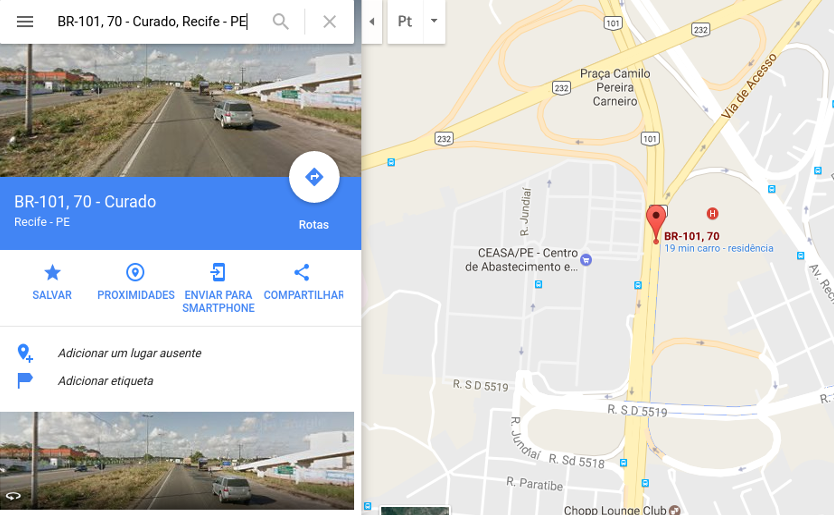
\includegraphics[width=110mm, height=65mm]{Figuras/Resultados/Km70BR101}\\
		\tiny Fonte: Google Maps
	\end{figure}
\end{frame}

\begin{frame}
	Correspondência entre AD e MM para o trecho em destaque
	\frametitle{M. Mortos: Km 56 -- 78, BR 101 (Sul)}
	\begin{figure}[htbp!]
		\centering
		\label{fig:MatrizMortos2d-101}
		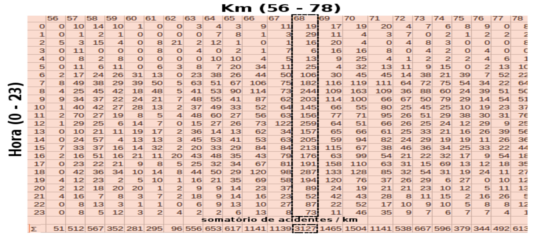
\includegraphics[width=110mm, height=50mm]{Figuras/Resultados/MM2d101}\\
		\tiny Fonte: o Autor
	\end{figure}
\end{frame}

\begin{frame}
	Sugestão de Roteamento: Goiana - Recife, a partir da Matriz de Gravidade 3D para 2ª-feira
	\begin{figure}[ht]
		\centering
		%\caption{Rota: Goiana - Recife, a partir da Matriz de Gravidade 3D para 2ª-feira}
		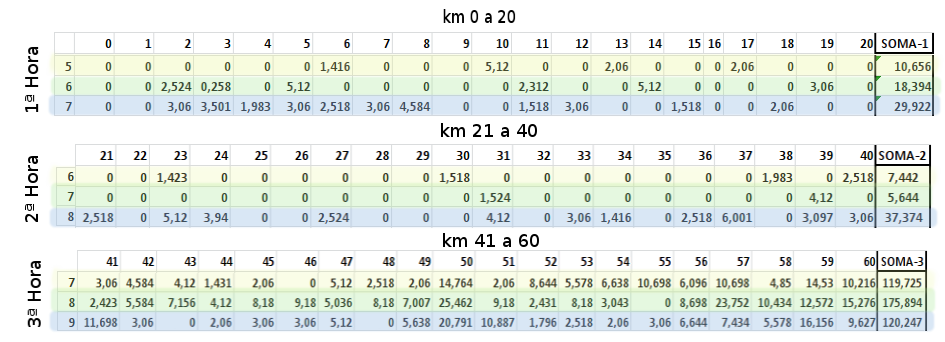
\includegraphics[width=110mm, height=60mm]{Figuras/Metodologia/RotaExemplo.png}\\
	\end{figure}
\end{frame}

\begin{frame}
	\frametitle{Aplicação da equação 3.1 para roteamentos}
	Três veículos partem do km 0 (zero) da BR 101 em horários diferente, segunda-feira, com destino ao Recife. O Veículo-x parte às 5h da manhã, o Veículo-y às 6h e o Veículo-z às 7h, eles percorrem com uma velocidade média de 20km/h.
	Resultados encontrado para os três veículos na mesma rota:
	 \begin{itemize}
	 	\item Veículo-x: 10,656 +  7,442 + 119,725 = 137,823
	 	\item Veículo-y: 18,394 +  5,644 + 175,894 = 199,932
	 	\item Veículo-z: 29,922 + 37,374 + 120,247 = 187.543
	 \end{itemize}
	Segundo os resultados acima, o Veículo-x chegara primeiro ao seu destino, seguido do Veículo-z e por último o Veículo-y.
\end{frame}


\subsection{Mineração em Textos no Twitter}
\begin{frame}
	\frametitle{Mineração de dados textuais}
	Minerar dados do Twitter demonstrou ser viável.
	O utilizador faz referências ao que acontece nas rodovias, podendo impactar em sua experiência ao utilizá-la.
	A figura a seguir são os termo mais frequentes capturados no canal @PRF191PE em um dia normal.
	\begin{figure}[ht]
		\centering
		%\caption{Rota: Goiana - Recife, a partir da Matriz de Gravidade 3D para 2ª-feira}
		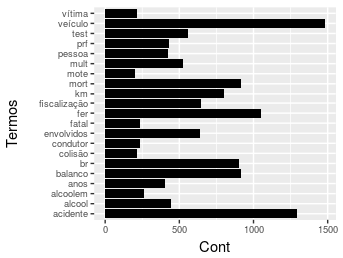
\includegraphics[width=75mm, height=45mm]{Figuras/Twitter/freqPalavr}\\
	\end{figure}
\end{frame}

\begin{frame}
	\frametitle{Mineração de dados textuais}
	O gráfico tipo Nuvem de palavras é outra maneira de se presentar as frequências de unigramas encontrados em outro dia comum no canal @PRF191PE.
	\begin{figure}[ht]
		\centering
		%\caption{Rota: Goiana - Recife, a partir da Matriz de Gravidade 3D para 2ª-feira}
		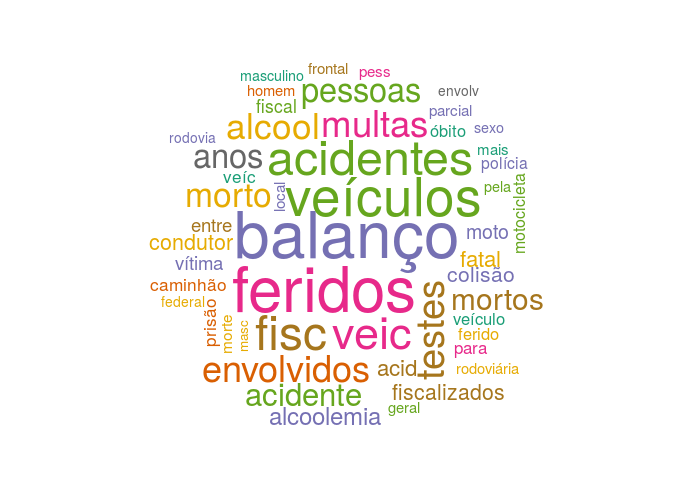
\includegraphics[width=75mm, height=45mm]{Figuras/Twitter/nuvem2.png}\\
	\end{figure}
\end{frame}


\begin{frame}
	\frametitle{Mineração de dados textuais}
	O dendograma é um gráfico que agrupa palavras de acorodo com o assunto. No dendograma a seguir destacamos os agrupamentos sobre o asssunto \textbf{colisão} com vítima fatal com um dos condutores estava em uma moto e houve prisão.
	\begin{figure}[ht]
		\centering
		%\caption{Rota: Goiana - Recife, a partir da Matriz de Gravidade 3D para 2ª-feira}
		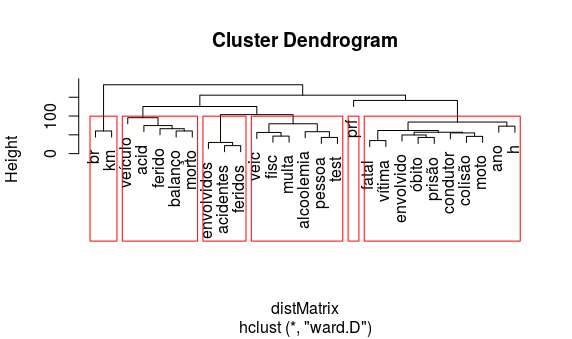
\includegraphics[width=75mm, height=45mm]{Figuras/Twitter/Cluster.png}\\
	\end{figure}
\end{frame}


\begin{frame}
	\frametitle{Mineração de dados textuais}
	O segundo gráfico de agrupamento demonstra a utilização do algorítmo K-means. Uma análise mais minuciosa desses gráficos podem trazer consideráveis contribuições ao modelo de predição da Etapa 2 da figura 4.1.
	\begin{figure}[ht]
		\centering
		%\caption{Rota: Goiana - Recife, a partir da Matriz de Gravidade 3D para 2ª-feira}
		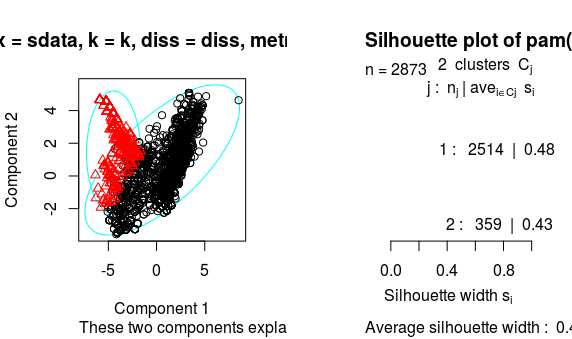
\includegraphics[width=95mm, height=35mm]{Figuras/Twitter/Cluster2.png}\\
	\end{figure}
\end{frame}
%++++++++++++++++++++++++++++++++++++++++++++++++++++++++++++++++++++++++++++++++++++++++++++++
\section{Conclusões}

\begin{frame}
	\frametitle{Considerações finais -- 1}
	O realização desta pesquisa sugere que é possível propor um modelo de predição que possibilite a gestão logística do ponto de vista do utilizador, em dias e horários mais convenientes, melhorando a experiência dos atores que fazem uso dessas rodovias.
	Resultados encontrados em outras pesquisas apontam a eficácia da utilização de I.A. para analisar e empregar soluções ao tráfego de veículos. 

\end{frame}


\begin{frame}
	\frametitle{Considerações finais -- 2}
	O dados encontrados sugerem que há um padrão de comportamento nas rodovias que pode ser analisado e predito pela I.A., de maneira a facilitar o tráfego de veículos e tornar as rodovias mais seguras.
	O registro pelo órgãos de trânsito tende a aumentar, oferecendo uma gama de opções para as pesquisas nessa área.
	Sentimos necessidade de informações de mais precisas sobre latitude e longitude, elas aparecem precariamente nos dados da PRF.
	Esta informação é de suma importância para pesquisadores e desenvolvedores que utilizam georreferenciamento. Por exemplo a BR 101, atravessa o país de norte a sul, em muitos trechos, em outros Estados o Km se repete.
	
\end{frame}

\begin{frame}
   \frametitle{Considerações finais -- 3}
   Uma das contribuições desta pesquisa é de cunho metodológico-prático. Destaca-se inicialmente pela articulação entre os resultados envolvendo diferentes algoritmos. A pesquisa utilizou Naïve Bayes, TF-IDF, Arvores de Decisão, Redes Neurais para o trabalho com os dados da PRF e do Twitter. Observa-se que isso parece ser uma tendência nos trabalhos que envolvem análise do tráfego em rodovias.
   Outra contribuição dessa pesquisa é a de unir predição e classificação, dados históricos a priori e dados de redes sociais a posteriori.

	
\end{frame}

\begin{frame}
	\frametitle{Considerações finais -- 4}
	Esta pesquisa também contribuiu para a compreensão das causas dos constantes constrangimentos e incidentes que paralisam as rodovias pernambucanas.
	Os dados revelam que o condutor é o principal causador e vítima dos danos registrados pela PRF e que a imprudência e desrespeito às leis são os maiores responsáveis pela grande quantidade de óbitos encontrados pois a esmagadora maioria dos acidentes ocorre em via reta, sem restrição de visibilidade com pista seca e em boas condições.
	
	Em análise restrita a morte por atropelamento, os dados sugerem concluir que não há uma estrutura segura que evite esse tipo de acidentes nem obrigue o pedestre a utilizar as passarelas de forma segura e eficiente.
	
\end{frame}

\begin{frame}
	\frametitle{Considerações finais -- 5}
  Outras condicionantes a acidentes nos perímetros urbanos, por exemplo, são falta de sinalização, passarelas, faixa de pedestres, barreiras de segurança, limitador de velocidades, dentre outros. A quantidade de acidentes que compreende o  trecho: km 66 ao km 71 da BR 101, com mais de 9 500 mortos por atropelamento nos últimos nove anos, aponta como o local mais perigoso para um pedestre atravessar no Estado de Pernambuco.
  
  O padrão de comportamento encontrado nesta pesquisa também foi encontrado em outras, neste país e em outros, já discutidas nesta dissertação, sugerindo que as variáveis relacionadas ao condutor são as mais fortes condicionantes de acidentes.  
	
\end{frame}

\begin{frame}
	\frametitle{Considerações finais -- 6}
	Ainda com relação à contribuição ao Estado da Arte descrito nesta Dissertação, esta pesquisa avança em relação ao que foi proposto em outros trabalhos ao identificar as ocorrências nas rodovias levando em conta o passado e o presente propondo um modelo que contemple o futuro possibilitando escolhas mais seguras e assertivas.
	
\end{frame}

%++++++++++++++++++++++++++++++++++++++++++++++++++++++++++++++++++++++++++++++++++++++++++++++

\section{Extras}
\subsection{Trabalhos futuros}

\begin{frame}
	\frametitle{Sistema de suporte a decisão}
	Trabalhos futuros sugerem ampliar as pesquisas a fim de propor o desenvolvimento de uma ferramenta que atenda a um gestor tomar decisões sobre a logística do transporte de cargas, utilizando os resultados encontrados, melhoramento modelo preditivo, incorporando novas técnicas para obter resultados melhores. 
	Ampliar a Equação 3.1 incorporando variáveis que permita com que uma equação do Momentum seja eficaz incorporando situações espaço-temporais ao integrar passado e futuro.

	
\end{frame}

\begin{frame}\frametitle{ Aplicativo}
	\transboxout[duration=2, direction=25]
	A fim de ampliar a utilização dessa pesquisa propomos aprimorar a etapa de extrapolação que culmine em um aplicativo para celulares. Uma breve sugestão de API é a figura a seguir. 
	\begin{figure}[ht]
		\centering
		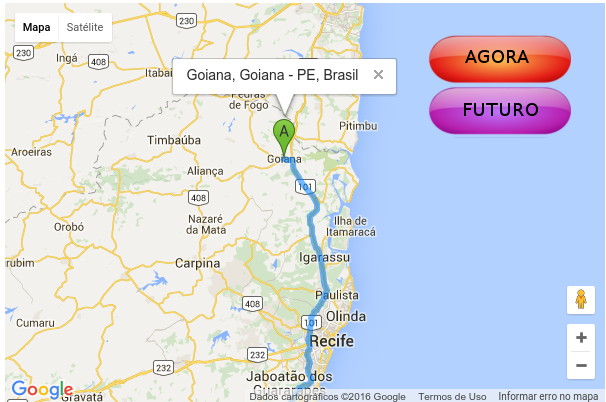
\includegraphics[width=100mm, height=45mm]{Figuras/Extras/InterfaceGrafica.png}
		\caption{ Interface Gráfica Proposta}		
	\end{figure}
\end{frame}

\subsection{Artigos aprovados em eventos} 
\begin{frame}\frametitle{ Artigo aprovado em evento internacional}
	\transboxout[duration=1, direction=25]
	\centering{ANÁLISE DE COMPORTAMENTO RODOVIÁRIO NA REGIÃO METROPOLITANA DO RECIFE-BRASIL -- UMA ABORDAGEM DE MINERAÇÃO DE DADOS}
	\begin{figure}[ht]
		\centering
		
\includegraphics[width=80mm, height=25mm]{Figuras/Extras/Cisti122.png}
		\caption{ CISTI -- Conf. Ibérica de Sistemas e Tecnologia da Informação}
	\end{figure}
\end{frame}

\end{document}
